% NOMS 2027 draft -- IEEEtran conference. Compile: pdflatex main; bibtex main; pdflatex main; pdflatex main
% Limite a confirmar na chamada do NOMS 2027 (NOMS 2023: 8 pp. + referências).
\documentclass[conference]{IEEEtran}
\usepackage[utf8]{inputenc}
\usepackage[T1]{fontenc}
\usepackage{cite,amsmath,amssymb,booktabs,array,xcolor,graphicx,tikz,url}
\usetikzlibrary{arrows.meta,positioning,fit}
\newcommand{\TODO}[1]{\textcolor{red}{[TODO: #1]}}
\newcommand{\TBD}{\textcolor{red}{TBD}}
\newcommand{\VER}{\textcolor{orange}{?}}   % célula da tabela ainda não verificada
\newif\ifanon \anonfalse
% valores padrão; generated/results_meta.tex (gerado pelo R) os redefine
\providecommand{\EOneRuns}{\TBD}\providecommand{\EOneLabel}{\TBD}
\providecommand{\ETwoRuns}{\TBD}\providecommand{\ETwoLabel}{\TBD}\providecommand{\EThreeRuns}{\TBD}\providecommand{\EThreeLabel}{\TBD}
\providecommand{\EOneMislabeled}{\TBD}\providecommand{\EOneFusedWrong}{\TBD}\providecommand{\EOneFusedUp}{\TBD}\providecommand{\EFiveLabel}{\TBD}\providecommand{\EFiveRuns}{\TBD}\providecommand{\EFiveConnAuto}{\TBD}\providecommand{\EFiveWrongAuto}{\TBD}\providecommand{\ESixLabel}{\TBD}\providecommand{\ESixRuns}{\TBD}\providecommand{\ESixDecAuto}{\TBD}\providecommand{\ESevenLabel}{\TBD}\providecommand{\ESevenRuns}{\TBD}\providecommand{\ESevenConn}{\TBD}\providecommand{\ESevenWrong}{\TBD}\providecommand{\ESevenDec}{\TBD}\providecommand{\ESevenDecOK}{\TBD}\providecommand{\ESevenFA}{\TBD}\providecommand{\ESevenFD}{\TBD}\providecommand{\ESevenND}{\TBD}\providecommand{\ESevenToolMs}{\TBD}\providecommand{\AgentnetdRuns}{\TBD}\providecommand{\AgentnetdEqual}{\TBD}\providecommand{\ETwoBLabel}{\TBD}\providecommand{\ETwoBRuns}{\TBD}\providecommand{\EThreeBLabel}{\TBD}\providecommand{\EThreeBRuns}{\TBD}\providecommand{\EOneFastCells}{\TBD}\providecommand{\EOneFastEqual}{\TBD}\providecommand{\EOneFastRuns}{\TBD}\providecommand{\EFourLabel}{\TBD}\providecommand{\EFourRuns}{\TBD}\providecommand{\EFourMCP}{\TBD}
\providecommand{\ResultsBanner}{}                   % \anontrue se a revisão for double-blind

\begin{document}
\title{Who Opened This Connection? Verifiable Per-Execution\\Network Accounting and Control for AI Agents}
\ifanon
\author{\IEEEauthorblockN{Anonymous Authors}}
\else
\author{\IEEEauthorblockN{Henrique Hermany, Jhonatan Jauja Ccana, Afonso Hafner de Britto,\\
Cec\'ilia Duarte Garcia, J\'eferson Campos Nobre, Eder John Scheid}
\IEEEauthorblockA{Institute of Informatics, Federal University of Rio Grande do Sul (UFRGS), Porto Alegre, Brazil\\
\{henrique.hermany, jjccana, ahbritto, ceciliad.garcia, jcnobre, ejscheid\}@inf.ufrgs.br}}
\fi
\maketitle

% ===== 00-abstract.tex =====
\begin{abstract}
AI agents turn model decisions into processes, subprocesses, and network connections. Network and service management needs to know which agent execution opened each connection, to account traffic per task and to scope egress policies, but the kernel sees connections, not executions. Existing eBPF-based agent systems rely on process lineage, cgroups, inherited task identifiers, or application bindings; each signal holds only under specific execution structures, and none of the systems we inspected fully provides both explicit ambiguity and validation against an independent reference. We present agentnet, a framework that fuses lineage, cgroup membership, and a runtime-provided execution identity while reporting ambiguity explicitly, binds that identity to the task rather than the thread so that it remains correct for asynchronous tools in a shared Model Context Protocol (MCP) server, and uses the same identity for live per-execution accounting and an in-kernel egress policy. Against a destination-based reference that shares no input with the system, fusion turns every faulty label into reported ambiguity when executions have distinct process trees; the task-scoped binding removes the misattributions that thread-keyed markers cause for asynchronous MCP tools, and the policy then makes no decision error; with concurrent LLM agents on a local model, attribution and policy decisions matched the reference. The collector adds 8 to 14\,$\mu$s per connection.
\end{abstract}

\begin{IEEEkeywords}
AI agents, eBPF, network accounting, observability, attribution, service management
\end{IEEEkeywords}

\section{Introduction}

Artificial intelligence (AI) agents built on large language models (LLMs) are moving beyond code generation into network and service management. Recent work applies them to the operation of beyond-5G and 6G networks~\cite{corici2025agents,xiao2025agentic}, to decentralized optimization of wireless networks~\cite{lee2025decentralized}, and to fault diagnosis in network management systems~\cite{chen2025assistant}. Delegating such tasks to agents can shorten reaction times and remove the human from routine operational loops.

However, this autonomy raises an accountability problem. AI agents do more than produce text: a single task can invoke tools, run shell commands, spawn subprocesses, and open network connections~\cite{yao2023react}, often without a human reviewing each step. In network operations, postmortems and compliance already require that agent decisions be auditable and replayable~\cite{martinezpaez2026vetra}. Agentic systems also widen the attack surface through prompt injection, tool misuse, and compromised components~\cite{chhabra2026agentic,ma2026openclaw}. In a red-teaming study, tool-enabled agents leaked sensitive data and ran destructive system actions~\cite{shapira2026chaos}. In a reported cyber-espionage campaign, an AI agent carried out most of the intrusion autonomously~\cite{anthropic2025espionage,dawson2026agentic}. Attributing such actions to the execution that performed them is a precondition for accountability, auditing, and containment. When agents run as shared services (\eg a Model Context Protocol (MCP)~\cite{mcp2025spec} server), several executions share a host, a container, or even a worker process. Thus, managing them as network consumers requires answering a simple question: \emph{which agent execution opened this connection?} The answer determines per-execution traffic accounting, the scope of egress policies, and the evidence available when an execution misbehaves.

One straightforward approach to monitoring the actions of such agents is to rely on kernel-level information, such as process creation, file accesses, and network connections, which an agent cannot avoid by switching tools, libraries, or wrappers~\cite{tetragon}. Further, recent technologies, such as the extended Berkeley Packet Filter (eBPF)~\cite{ebpf}, make this practical by attaching verified programs to kernel events, such as process creation and socket operations, without modifying the kernel or the monitored applications~\cite{gbadamosi2024ebpf}. However, the kernel sees connections, processes, and control groups (\textit{cgroups}), but not tasks or tool calls. 

Recent eBPF-based agent systems bridge this gap with different signals: process lineage and temporal correlation~\cite{zheng2025agentsight}, cgroups aligned with tool calls~\cite{zheng2026agentcgroup}, bindings between application context and runtime facts~\cite{byteyellow2026agentprovenance}, inherited task identifiers~\cite{cui2026contractwarden}, and policy domains or tracked process scopes for enforcement~\cite{zheng2026actplane,shukla2026agentguard}. Each signal is informative only under specific execution structures. In a shared \textit{cgroup}, membership cannot separate concurrent executions; inside a shared worker, neither cgroup nor lineage can. Recent work still describes per-tool-call attribution as an open problem~\cite{king2026kernelevidence}.

To address such an open problem, this paper presents \solution{} (Fused Attribution, Accounting, and Control per Task), a framework that attributes each network connection to the agent execution that opened it, reports ambiguity explicitly when the available signals cannot separate executions, and uses the resulting identity for per-execution management. In summary, the contributions of this paper are two-fold: \1 a task-level attribution mechanism that fuses runtime identity, process lineage, and cgroup membership and remains correct for asynchronous tools in shared MCP servers; and \2 per-execution accounting and kernel-enforced egress control on the same identity. Experiments with a real MCP server, a real network interface, and LLM agents driven by open and commercial models show that \solution{} attributes every connection correctly, whereas an existing system misattributes up to 96\% of them, at a cost of microseconds per connection.

The remainder of this paper is organized as follows: Section~\ref{sec:background} provides the background on the involved topics, Section~\ref{sec:related} reviews related work, Section~\ref{sec:design} presents \solution, Section~\ref{sec:method} describes the methodology, Section~\ref{sec:results} reports the results, Section~\ref{sec:discussion} discusses limitations, and Section~\ref{sec:conclusion} concludes this paper.
% ===== 02-background.tex =====
\section{Background}
\label{sec:background}
\textbf{Agent executions.} An agent runtime (harness) drives a loop in which a language model selects tools; each invocation is a \emph{tool call}, and the steps devoted to one goal form a \emph{task}~\cite{yao2023react}. In this paper, an \emph{execution} is the semantic unit to which network activity should be attributed. Its correspondence to operating-system entities depends on how the runtime organizes work: one execution may spawn many processes, and one worker process may serve many executions.

\textbf{Kernel identity signals.} A PID identifies the task that issues a system call. \emph{Process lineage} associates descendants with the root of an execution tree; it discriminates executions only while they live in distinct trees. \emph{Cgroups} group processes for accounting and resource control; their membership discriminates executions only when the group layout separates them~\cite{zheng2026agentcgroup}. \emph{Application context}, such as session, task, or tool-call identifiers, can be bound to runtime facts~\cite{byteyellow2026agentprovenance,otel2026genai}. It can represent distinctions absent from the process structure, but its correctness depends on the binding.

\textbf{Attribution outcomes.} We classify the resolver output for each observed event against a reference origin: \emph{correct} (C) when the single selected origin matches the reference; \emph{ambiguous} (A) when the output is a set of candidates; \emph{missing} (M) when no origin is assigned; and \emph{incorrect} (I) when the single selected origin differs from the reference. For management, I is the costly outcome: it credits traffic to the wrong execution without warning. A, by contrast, is visible and can be handled by policy.

\section{Related Work}
\label{sec:related}
Prior work relates agent activity to operating-system events for observability and provenance, resource control and enforcement, general-purpose instrumentation, and request accounting. We review it in this order and then compare it along the dimensions that network attribution requires.

AgentSight~\cite{zheng2025agentsight} correlates intercepted LLM traffic with kernel events through process lineage, a 100--500\,ms temporal window, and argument matching. Its network events are per-process summaries, and its evaluation reports overhead and case studies, not correlation accuracy. AgentProvenance~\cite{byteyellow2026agentprovenance} is the closest system: it resolves syscall-level \texttt{connect} events to execution-scope and tool-call bindings through cgroup, process, and time tiers, and it marks unmatched events as \emph{unresolved}. However, its events carry no connection identity, overlapping bindings are resolved silently (latest start wins) rather than reported as ambiguous, and its validation consists of pass/fail acceptance tests. King et al.~\cite{king2026kernelevidence} validate kernel evidence at session level and state explicitly that per-tool-call attribution remains an open problem.

AgentCgroup~\cite{zheng2026agentcgroup} places each shell tool call in its own cgroup for CPU and memory control; it does not account network activity. ActPlane~\cite{zheng2026actplane} and AgentGuard~\cite{shukla2026agentguard} enforce network policies over process-tree domains or tracked PIDs; AgentGuard keys denied connections to a single globally active session. ContractWarden~\cite{cui2026contractwarden} stores a task identifier in BPF task-local storage, inherited across fork and exec, and enforces policies at \texttt{socket\_connect}; its unit is the launched task, not the individual tool call, and it does not report ambiguity or validate attribution. IsolateGPT~\cite{wu2025isolategpt} isolates the apps of an agent system in separate execution environments, and Progent~\cite{shi2025progent} enforces privilege policies on tool calls inside the agent; neither attributes the resulting kernel network activity.

OpenTelemetry eBPF Instrumentation (OBI)~\cite{otel2026obi} produces HTTP/gRPC spans with W3C trace-context propagation across threads and event loops, and exports flow metrics labeled with workload attributes. In the inspected source, context does not follow forked children and flow metrics carry no request identity. DeepFlow~\cite{shen2023deepflow} assembles distributed traces from eBPF-captured network messages without code changes, and Tetragon~\cite{tetragon} enforces process-aware policies in the kernel; both key activity to processes, containers, or protocol-level requests, not to agent executions. The OpenTelemetry GenAI conventions define a tool-call identifier at the application level~\cite{otel2026genai}, which kernel network events do not carry.

Charging kernel activity to logical requests predates agents: resource containers decouple accounting from processes~\cite{banga1999resource}; Magpie and Whodunit reconstruct requests from kernel and inter-process events~\cite{barham2004magpie,chanda2007whodunit}; X-Trace, Dapper, Canopy, Pivot Tracing, and Retro propagate request context for tracing and per-workflow resource management~\cite{fonseca2007xtrace,sigelman2010dapper,kaldor2017canopy,mace2015pivot,mace2015retro}; and provenance systems capture whole-system provenance in the kernel~\cite{pasquier2017camflow}, partition long-running processes into units~\cite{lee2013beep,ma2017mpi}, or fuse application and audit logs~\cite{hassan2020omegalog,yu2021alchemist}. We build on these ideas; our contribution is their combination for agent tool calls, including subprocesses and non-HTTP Transmission Control Protocol (TCP) connections, with explicit ambiguity and an independent reference.

We compare these efforts along eight dimensions that network attribution requires: \textbf{D1} kernel-level data capture (\eg with eBPF); \textbf{D2} process lineage; \textbf{D3} cgroup membership; \textbf{D4} binding of application context to kernel facts; \textbf{D5} attribution of network activity at connection or flow granularity; \textbf{D6} explicit ambiguity in the output (\ie reporting several candidates rather than forcing a choice); \textbf{D7} validation of attribution against an independent reference; and \textbf{D8} a per-execution management action (\eg accounting or policy). D2 and D3 separate executions with distinct trees or groups. D4 is the only source of distinction inside a shared worker. D5 links traffic, rather than only processes, to executions. D6 and D7 determine whether the output can be trusted for management decisions.

\begin{table}[t]
\centering
\caption{Coverage of attribution dimensions}
\label{tab:dims}
\footnotesize
\setlength{\tabcolsep}{2.6pt}
\begin{tabular*}{\columnwidth}{@{\extracolsep{\fill}}lcccccccc@{}}
\toprule
\textbf{Work} & \textbf{D1} & \textbf{D2} & \textbf{D3} & \textbf{D4} & \textbf{D5} & \textbf{D6} & \textbf{D7} & \textbf{D8} \\
\midrule
AgentSight~\cite{zheng2025agentsight} & \checkmark & \checkmark & $\circ$ & $\circ$ & $\times$ & $\times$ & $\times$ & $\times$ \\
AgentCgroup~\cite{zheng2026agentcgroup} & $\circ$ & $\times$ & \checkmark & $\circ$ & $\times$ & $\times$ & $\times$ & $\circ$ \\
AgentProvenance$^\dagger$~\cite{byteyellow2026agentprovenance} & \checkmark & $\circ$ & \checkmark & \checkmark & $\circ$ & $\circ$ & $\circ$ & $\circ$ \\
ActPlane~\cite{zheng2026actplane} & \checkmark & \checkmark & $\times$ & $\times$ & $\times$ & $\times$ & $\times$ & \checkmark \\
AgentGuard~\cite{shukla2026agentguard} & \checkmark & \checkmark & $\times$ & $\circ$ & $\circ$ & $\times$ & $\times$ & \checkmark \\
ContractWarden~\cite{cui2026contractwarden} & \checkmark & $\circ$ & \checkmark & $\circ$ & $\circ$ & $\times$ & $\times$ & \checkmark \\
OTel eBPF (OBI)~\cite{otel2026obi} & \checkmark & $\circ$ & $\times$ & $\circ$ & $\circ$ & $\times$ & $\times$ & $\circ$ \\
\textbf{\solution{} (this work)} & \checkmark & \checkmark & \checkmark & \checkmark & \checkmark & \checkmark & \checkmark & \checkmark \\
\bottomrule
\end{tabular*}
\scriptsize
\checkmark: present; $\circ$: partial or by other means; $\times$: no evidence in inspected sources; $^\dagger$: also confirmed by running the system (E5ap)
\end{table}

We assessed each system using its published design, documentation, and source code, and marked a dimension only when the inspected sources show the capability (\cf Table~\ref{tab:dims}). Most systems capture kernel events and use process lineage or cgroups (D1--D3), but none reports a candidate set when these signals cannot separate executions; AgentProvenance only marks unmatched events as unresolved (D6). Only AgentProvenance partially validates attribution, through acceptance tests rather than an independent reference (D7). Running it (E5ap, Section~\ref{sec:results}) confirmed its marks: overlapping bindings were resolved to the latest one without reporting ambiguity (D6), and connections of child processes were matched only in part (D2). Network activity is attributed per connection only partially (D5), and the systems that act per execution (D8) key their decisions to process trees, tracked PIDs, or launched tasks rather than to individual tool calls. \solution{} covers all eight dimensions and is the only one that reports ambiguity explicitly and validates attribution against an independent reference.

\section{\solution~Design}
\label{sec:design}

Fig.~\ref{fig:arch} depicts the components of \solution. It is composed of a runtime binding that ties each tool call to its execution, a kernel collector, a fusion resolver, a live accounting daemon, and a per-execution egress policy that uses the same~identity.

\begin{figure}[!h]
\centering
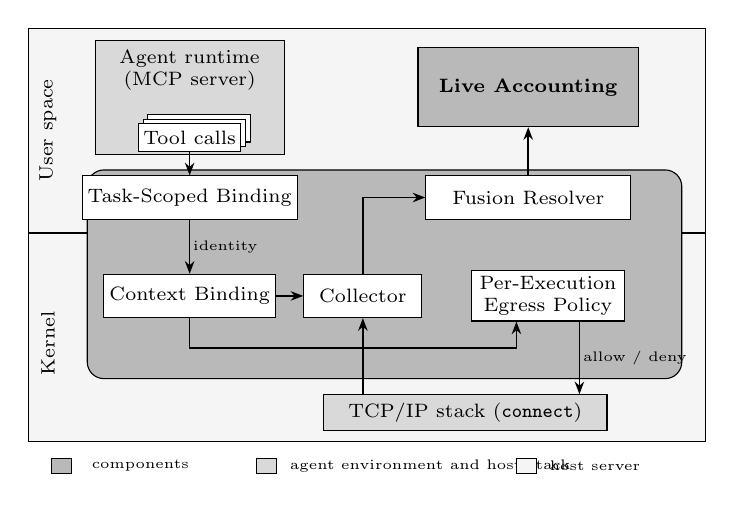
\begin{tikzpicture}[font=\scriptsize, x=1cm, y=1cm,
  comp/.style={draw, fill=white, align=center, inner sep=2pt, minimum height=5.5mm},
  env/.style={draw, fill=gray!30, align=center, inner sep=2pt},
  arr/.style={-{Stealth[length=1.6mm]}, semithick},
  lab/.style={font=\tiny, inner sep=1pt}]
\draw[fill=gray!8] (0,-0.25) rectangle (8.6,5.0);
\draw (0,2.4) -- (8.6,2.4);
\node[rotate=90] at (0.25,3.7) {User space};
\node[rotate=90] at (0.25,1.0) {Kernel};
\node[env, minimum width=2.4cm, minimum height=1.45cm, anchor=north] (rt) at (2.05,4.85) {};
\node[anchor=north, align=center] at (rt.north) {Agent runtime\\(MCP server)};
\node[comp, minimum width=1.3cm, minimum height=3.5mm, inner sep=1pt] at (2.17,3.73) {};
\node[comp, minimum width=1.3cm, minimum height=3.5mm, inner sep=1pt] at (2.11,3.67) {};
\node[comp, minimum width=1.3cm, minimum height=3.5mm, inner sep=1pt] (tc) at (2.05,3.61) {Tool calls};
\node[comp, fill=gray!55, font=\scriptsize\bfseries, minimum width=2.8cm, minimum height=1.0cm] (la) at (6.35,4.25) {Live Accounting};
\draw[rounded corners=6pt, fill=gray!55] (0.75,0.55) rectangle (8.3,3.2);
\node[font=\scriptsize\bfseries, anchor=south west] at (0.85,0.6) {\solution};
\node[comp, minimum width=2.0cm] (tsb) at (2.05,2.85) {Task-Scoped Binding};
\node[comp, minimum width=2.6cm] (fr) at (6.35,2.85) {Fusion Resolver};
\node[comp, minimum width=1.75cm] (cb) at (2.05,1.6) {Context Binding};
\node[comp, minimum width=1.5cm] (col) at (4.25,1.6) {Collector};
\node[comp, minimum width=1.95cm, align=center] (pol) at (6.6,1.6) {Per-Execution\\Egress Policy};
\node[env, minimum width=3.6cm, minimum height=4.5mm] (tcp) at (5.55,0.12) {TCP/IP stack (\texttt{connect})};
\draw[arr] (tc) -- (tsb);
\draw[arr] (tsb) -- node[lab, right]{identity} (cb);
\draw[arr] (cb) -- (col);
\draw[arr] (cb.south) -- ++(0,-0.38) -| ([xshift=-4mm]pol.south);
\draw[arr] (col.north) |- (fr.west);
\draw[arr] (fr) -- (la);
\draw[arr] (tcp.north -| col) -- (col.south);
\draw[arr] ([xshift=4mm]pol.south) -- node[lab, right]{allow / deny} ([xshift=4mm]pol.south |- tcp.north);
\begin{scope}[shift={(0.3,-0.65)}, every node/.style={font=\tiny, anchor=west}]
\draw[fill=gray!55] (0,0) rectangle +(0.25,0.18); \node at (0.3,0.09) {\solution{} components};
\draw[fill=gray!30] (2.6,0) rectangle +(0.25,0.18); \node at (2.9,0.09) {agent environment and host stack};
\draw[fill=gray!8] (5.9,0) rectangle +(0.25,0.18); \node at (6.2,0.09) {host server};
\end{scope}
\end{tikzpicture}
\caption{\solution{} architecture.}
\label{fig:arch}
\end{figure}

\subsection{Collector}

eBPF programs record, for every thread, \texttt{sched\_process\_fork}, \texttt{exec}, and \texttt{exit}, from which lineage is reconstructed. They also hook \texttt{tcp\_connect} in process context, capturing PID, thread ID, cgroup v2 ID, current context, and socket. The handshake outcome is taken from \texttt{inet\_sock\_set\_state} and joined by socket. Socket state changes may run in softirq context, so the PID observed there is never used for attribution.

\subsection{Context Binding}

The runtime hands the execution identity to the kernel through markers that the collector records in a kernel map keyed by thread ID; on fork or thread creation, the child inherits the parent's entry, so a tool that runs as a subprocess carries the identity without any change to the tool. In the prototype, a marker is an \texttt{openat} call on a reserved, nonexistent path, captured by a tracepoint; it needs no library and costs one failed system call. Emitting markers only at the start and end of each tool call (\emph{manual binding}) is correct for blocking, threaded, and subprocess tools, but not for asynchronous ones: coroutines of different executions interleave on the event-loop thread and overwrite its entry (Section~\ref{sec:results}).

\subsection{Task-Scoped Binding}
\texttt{fact\_rt} makes the binding follow the task instead of the thread. The execution identity is stored in a context variable, which the asynchronous runtime copies into every task and into worker threads. In Python, the library wraps \texttt{socket.connect}/\texttt{connect\_ex} and process creation (\texttt{subprocess.Popen} and \texttt{os.fork}) and, immediately before the system call, sets the calling thread's kernel entry to the identity of the current task, or clears it if the task has none. Because no other coroutine can run between the marker and the system call, each connection and each child process carries the identity of the task that created it, regardless of interleaving. The entry is not cleared after the call; a connection that bypasses these wrappers (\eg from native code) inherits the identity of the last task that connected on that thread, a limitation we discuss in Section~\ref{sec:discussion}. For MCP servers, a wrapper around the \texttt{tools/call} handler takes the identity from the request's \texttt{\_meta} field, which the protocol reserves for metadata, and binds it for the duration of the call, so tool code is unmodified.

\subsection{Fusion Resolver}
For each connection the resolver receives only $(t, \mathit{pid}, \mathit{tid}, \mathit{cgroup}, \mathit{ctx})$ and computes three candidate sets: $L$ from the nearest registered lineage root, $G$ from the cgroup registry, and $c$ from the context binding. Let $S$ be the intersection of the non-empty structural sets, or their union if they are disjoint (structural conflict). The output is:
\begin{itemize}
  \item $\{c\}$ if a context is present and $S=\emptyset$ or $c \in S$;
  \item $S \cup \{c\}$ (ambiguous) if a context is present and $c \notin S$, \ie the context contradicts the process structure;
  \item $S$ otherwise, which may be a single origin, a candidate set, or empty.
\end{itemize}
The resolver never selects among candidates that the available information cannot separate. When the structure is informative (distinct trees), a mislabeled context therefore becomes ambiguity rather than misattribution. When the structure is uninformative (a shared worker), correctness rests entirely on the binding.

\subsection{Live Accounting}
\texttt{factd} consumes the collector stream, reorders events from different CPUs within a short window, applies the same fusion function as the offline evaluation, and periodically exports one flow-like record per execution, in the format of IP Flow Information Export (IPFIX)~\cite{rfc7011} (\ie connections, established, failed, distinct destinations), plus the ambiguous and unattributed counts with their candidate sets. Ambiguous or unattributed connections are never credited to an execution.

\subsection{Per-Execution Egress Policy}

A \texttt{cgroup/connect4} eBPF program, loaded with libbpf, keeps its own copy of the per-thread identity map (fed by the same markers) and decides each Internet Protocol version 4 (IPv4) \texttt{connect} by looking up the pair (execution, destination) in an allow-list map; connections without identity receive a configurable default action (\textit{deny} in our experiments), instead of inheriting a guess. Every decision is logged to a ring buffer for auditing. Thus, policy and accounting share one notion of identity, and errors in the binding become measurable policy errors: a false allow is a policy bypass and a false \textit{deny} is a loss of availability. The policy also applies the resolver's lineage check in the kernel. The launcher registers the root of every process tree that belongs to a single execution, and the root is inherited on fork and thread creation. When a thread's label contradicts the owner of its tree, the default mode denies the connection and logs a conflict; an alternative mode decides by the tree owner. A tree shared by several executions (a shared worker) is not registered, so there the decision follows the label.

\section{Evaluation Methodology}
\label{sec:method}

We measure a real system under a controlled workload~\cite{jain1991art}; factorial designs, randomization, and blocking follow standard experimental design~\cite{montgomery2017design}. The measured host is a VMware virtual machine (8 vCPUs of a Xeon Platinum 8276M, one NUMA node, 16\,GB, vmxnet3) running Linux 7.0 and bpftrace 0.25; some experiments add an identical second one on the same physical host and virtual switch, with an NVIDIA RTX~3060 (12\,GB) serving Ollama 0.40.6.

\subsection{Workloads and Reference}

Synthetic executions run under four conditions: \textbf{N0} distinct process trees and distinct cgroups (control); \textbf{N1} distinct trees sharing one cgroup v2, running concurrently; \textbf{N2} one worker process serving operations of all executions sequentially in random order; and \textbf{N3} one worker serving them concurrently on a pool of 8 threads. Each operation is marked with the runtime context marker and opens a TCP connection, either in the execution's own thread (\emph{inproc}) or through a forked and exec'd subprocess (\emph{subproc}), so that context inheritance across process boundaries is exercised.

Before each run, every operation is assigned an exclusive local destination port, drawn at random and stored in the run plan. The reference origin of a captured connection is obtained from its destination. Resolvers receive only $(t, \mathit{pid}, \mathit{tid}, \mathit{cgroup}, \mathit{ctx})$, and a static check over the resolver code rejects any reference to destination fields. The reference therefore shares no input with the signals under evaluation, \ie it is an oracle independent of the system under test~\cite{barr2015oracle}. Connections to ports outside the plan are counted and excluded; planned operations without a captured connection are reported as capture loss.

The four resolvers (cgroup-only, lineage-only, context-only, and fused) are applied offline to the same event log of each run, so differences between resolvers cannot come from different executions. The same logs feed emulations of the mechanisms of related systems (\cf Section~\ref{sec:results}).

To inject faults, a fraction $p \in \{0, 0.05, 0.2\}$ of each execution's operations is labeled with another execution's identifier, modeling runtime bugs in the context binding, following controlled fault-injection practice~\cite{arlat1990fault,hsueh1997fault}. The number of mislabeled operations is exact ($p \times$ operations), with positions drawn at random, so that fault injection adds no sampling variance.

\subsection{Experiments}
\textbf{E1} (correctness) is a full factorial over structure (N0--N3), $p$, and operation mode, with two executions of 100 operations each. \textbf{E2} (scale) varies the number of concurrent executions ($K \in \{2,4,\dots,64\}$) and the connection rate, with a random pause of up to 10\,ms between connections (\emph{paced}) or none (\emph{max}), in N1 and N3; \textbf{E2b} (capacity) runs $P$ concurrent instances of the closed-loop \texttt{connect} microbenchmark of E3 to find where capture stops being complete. \textbf{E3} (overhead) measures \texttt{connect} latency and throughput with that C microbenchmark, with and without the collector and the context markers, and \textbf{E3b} splits this cost across four configurations: no instrumentation, probes that only count events, the full collector, and an optimized collector. \textbf{E1fast} reruns E1 with the optimized collector to check that its outcomes do not change.

The next experiments use a real Model Context Protocol server, built with FastMCP, the official Python software development kit (SDK), over Server-Sent Events. In \textbf{E4}, $K \in \{2,4\}$ client sessions share it and issue 25 tool calls each; the tool runs synchronously, in a worker thread, as a subprocess, or as an \texttt{async} coroutine, and emits markers at its start and end. \textbf{E5} compares this manual binding with the task-scoped binding on the same server and tools, with $K \in \{2,4,8\}$; in the automatic mode the tools emit no markers and the identity travels in \texttt{\_meta}. \textbf{E6} adds the egress policy. Executions alternate between a permissive class (all planned destinations) and a restricted one (a random half of its own), so a mislabel can cause both false allows and false denies. In \textbf{E7}, four LLM agents (Qwen2.5-3B served locally by Ollama, temperature 0) perform health-check tasks through a shared, instrumented MCP server with HTTP, subprocess, and TCP-check tools, with the policy active; the model, not a script, decides which tools to call. \textbf{E7m} repeats E7 with Qwen2.5-7B and Llama-3.1-8B on the GPU of the second machine and with four and eight agents. \textbf{E7c} and \textbf{E7o} use commercial models from two leading providers, a high-end and an entry-level tool-calling model of each: Anthropic's Claude Opus~5.5 and Haiku~5.5 (Messages API) and OpenAI's GPT-6.1 Sol and GPT-6 Luna (Responses API, reasoning effort \emph{low}). \textbf{E7r} replays every recorded E7c and E7o run without models (same calls, arguments, labels, and timing).

Finally, \textbf{E5f}, \textbf{E6f}, and \textbf{E7f} repeat E5--E7 with the task-scoped binding while a fraction $p \in \{0.04, 0.2\}$ of each execution's tool calls carries another execution's identity (in E7f, one of each agent's first three calls). \textbf{E6L} runs the policy in N0 and N1 with $p \in \{0.05, 0.2\}$ and three lineage modes (label only, deny on conflict, tree owner), and \textbf{E6Ls} checks, in the shared MCP server without faults, that the lineage check never vetoes a correct label.

\textbf{E5net}, \textbf{E6net}, and \textbf{E3net} repeat E5, E6, and E3 with the services on the second machine, so connections leave through the virtual network interface instead of loopback. In \textbf{E5ap}, AgentProvenance~v0.9.0~\cite{byteyellow2026agentprovenance} runs next to \solution{} in the E5 rounds: its eBPF sensor captures the same connections, we register one binding per tool call as its harness integrations do (call, session, the MCP server's process and cgroup, and the call window seen by the client), and its own engine assigns each connection, scored against the same reference.

\subsection{Metrics and Analysis}
For connections with a valid reference: C/N, A/N, M/N, I/N, and C/(C+I) per resolver (\cf Section~\ref{sec:background}). For accounting, each execution's connections are split into correctly credited, credited to a wrong execution, and uncredited (ambiguous or missing). We do not report the net accounting error alone, because opposite misattributions cancel in it. For E3: median and 99th-percentile latency, throughput, and eBPF nanoseconds per program run.

The unit of repetition is a complete run, with a fresh collector process, new cgroups, and new services; events within a run are not independent replicates~\cite{georges2007statistically}. Run order is randomized with a recorded seed against ordering bias~\cite{mytkowicz2009producing}, and a repetition uses the same seed in every cell (common random numbers). Boots are treated as a higher level of variation~\cite{kalibera2013rigorous}: E1, E2b, E3, E3b, E5--E7, their network, model, and AgentProvenance variants, and the fault-injection experiments are spread over two boots. The sample size depends on the type of claim. For properties expected to hold exactly (I=0 in E5--E7), the primary result is the number of runs with any error; as a secondary summary we give the one-sided 95\% Clopper--Pearson upper bound on the per-connection error rate~\cite{clopper1934use}, about $3/n$ with zero errors in $n$ cases~\cite{hanley1983nothing}, so we planned at least 299 cases per cell (a 1\% bound): 6 runs per cell in E5, E6, and their variants, and 26 per E7, E7m, E7c, and E7o cell, counted on decisions; for AgentProvenance, 300 or more connections per cell give a 95\% interval of $\pm$5.7 points. It assumes independent connections, which does not strictly hold within a run. For performance (E3, E3b, E3net), runs per boot are sized from the pilot variance for a 95\% confidence-interval half-width of 5\%~\cite{hoefler2015scientific}. E1 is deterministic given the labels and is reported as counts. Every campaign used here is \emph{confirmatory}: it ran from a clean revision after a passing preflight, with no failed run; pilots are never results.

\subsection{Reproducibility}
\label{sec:repro}

User tools (Python, R, Snakemake) are pinned by a Nix flake; the kernel, bpftrace, and bpftool are recorded per campaign. A Snakemake workflow and one script per boot run preflight, campaigns, validation, and report. Each campaign is an immutable directory with run order, raw events, plans, scores, environment snapshots, git revision, manifest, and SHA-256 checksums, and every table and figure is generated by script from these directories~\cite{bajpai2019dagstuhl,collberg2016repeatability}.
The code and workflow and summarized results are available at~\cite{sourceCode}.

\section{Results}
\label{sec:results}
% generated by analysis/analysis.R: provenance of the paper's numbers
\def\EOneMislabeled{1200}
\def\EOneFusedWrong{0}
\def\EOneFusedUp{0.25}
\def\EOneLabel{confirmatory}
\def\EOneRuns{144}
\def\EOneCampaigns{hermes-E1-confirmatory-20261012T053433Z, hermes-E1-confirmatory-20261012T054704Z}
\def\ETwoLabel{confirmatory}
\def\ETwoRuns{120}
\def\EThreeLabel{confirmatory}
\def\EThreeRuns{40}
\def\EOneFastCells{96}
\def\EOneFastEqual{96}
\def\EOneFastRuns{24}
\def\EFourLabel{confirmatory}
\def\EFourRuns{40}
\def\EFourMCP{1.6.0}
\def\EFiveLabel{confirmatory}
\def\EFiveRuns{144}
\def\EFiveConnAuto{8400}
\def\EFiveWrongAuto{0}
\def\ESixLabel{confirmatory}
\def\ESixRuns{96}
\def\ESixDecAuto{6000}
\def\ESevenLabel{confirmatory}
\def\ESevenRuns{26}
\def\ESevenConn{260}
\def\ESevenWrong{0}
\def\ESevenDec{312}
\def\ESevenDecOK{312}
\def\ESevenFA{0}
\def\ESevenFD{0}
\def\ESevenND{0}
\def\ESevenToolMs{9}
\def\EThreeBLabel{confirmatory}
\def\EThreeBRuns{80}
\def\ETwoBLabel{confirmatory}
\def\ETwoBRuns{100}
\def\AgentnetdRuns{594}
\def\AgentnetdEqual{594}
\def\EFiveNetLabel{confirmatory}
\def\EFiveNetRuns{144}
\def\EFiveNetConnAuto{8544}
\def\EFiveNetWrongAuto{0}
\def\EFiveNetCapture{16800}
\def\EFiveNetAttempted{16800}
\def\EFiveNetAsyncManMin{7}
\def\EFiveNetAsyncManMax{30}
\def\EFiveNetMaxDiff{4}
\def\ESixNetLabel{confirmatory}
\def\ESixNetRuns{96}
\def\ESixNetDecAuto{6000}
\def\ESixNetErrAuto{0}
\def\ESevenMLabel{confirmatory}
\def\ESevenMRuns{104}
\def\ESevenMConn{2134}
\def\ESevenMWrong{0}
\def\ESevenMAmb{0}
\def\ESevenMDec{1872}
\def\ESevenMDecOK{1872}
\def\ESevenMFA{0}
\def\ESevenMFD{0}
\def\ESevenMND{0}
\def\ESevenMToolMs{10}
\def\ESevenCLabel{confirmatory}
\def\ESevenCRuns{104}
\def\ESevenCConn{1560}
\def\ESevenCWrong{0}
\def\ESevenCAmb{0}
\def\ESevenCDec{1872}
\def\ESevenCDecOK{1872}
\def\ESevenCUSD{4.60}
\def\ESevenCInTok{1952}
\def\ESevenCOutTok{280}
\def\ESevenOLabel{confirmatory}
\def\ESevenORuns{104}
\def\ESevenOConn{1560}
\def\ESevenOWrong{0}
\def\ESevenOAmb{0}
\def\ESevenODec{1872}
\def\ESevenODecOK{1872}
\def\ESevenOUSD{0.86}
\def\ESevenOInTok{730}
\def\ESevenOOutTok{117}
\def\ESevenOReasTok{1}
\def\ESevenRRuns{416}
\def\ESevenRSame{416}
\def\ESevenRCalls{416}
\def\ESevenRConn{6240}
\def\ESevenRWrong{0}
\def\ESevenRDec{7488}
\def\ESevenRDecOK{7488}
\def\EThreeNetLabel{confirmatory}
\def\EThreeNetRuns{40}
\def\EThreeNetBase{59}
\def\EThreeNetAdd{12.2}
\def\EThreeNetAddMk{20.2}
\def\EThreeNetRel{21}
\def\APRuns{72}
\def\APConn{8400}
\def\APWrongMin{92}
\def\APWrongMax{96}
\def\APWrongTwoMin{54}
\def\APWrongTwoMax{92}
\def\APSubMin{7}
\def\APSubMax{58}
\def\APAgentnetWrong{0}
\def\APAgentnetConn{8400}
\def\ResultsBanner{}

\IfFileExists{generated/baselines_meta.tex}{% generated by analysis/baselines_table.py
\def\BaseRuns{60}
\def\BaseCampaigns{hermes-E1-confirmatory-20261012T053433Z, hermes-E1-confirmatory-20261012T054704Z, hermes-E5-confirmatory-20261012T181111Z, hermes-E5-confirmatory-20261012T195813Z}
\def\BaseNearErrEveryRun{yes}
\def\BaseOursWrong{0}
}{\def\BaseRuns{\TBD}}
\IfFileExists{generated/fault_meta.tex}{% generated by analysis/fault_tables.py
\def\FaultEsevenMis{104}
\def\FaultEsevenFA{0}
\def\FaultEsevenAllowed{0}
\def\FaultEsevenFD{86}
\def\FaultEsevenRuns{26}
\def\FaultEsevenOther{0}
\def\FaultEfiveRuns{128}
\def\FaultEsixRuns{128}
\def\FaultConn{16000}
\def\FaultMis{1920}
\def\FaultMisWrong{1920}
\def\FaultSpill{0}
\def\FaultPolMis{1920}
\def\FaultPolErr{1112}
\def\FaultPolErrPct{58}
\def\LinRuns{96}
\def\LinConflictsExact{yes}
\def\LinModeTwoErr{0}
\def\LinModeTwoDec{6400}
\def\LinModeOneFA{0}
\def\LinModeZeroErr{592}
\def\LinModeZeroMis{800}
\def\LinModeZeroPct{74}
\def\LsRuns{48}
\def\LsDecisions{6000}
\def\LsErrors{0}
\def\LsConflicts{0}
\def\FaultCampaigns{hermes-E5f-confirmatory-20261013T024326Z, hermes-E5f-confirmatory-20261013T033751Z, hermes-E6L-confirmatory-20261013T023556Z, hermes-E6L-confirmatory-20261013T033021Z, hermes-E6Ls-confirmatory-20261013T023941Z, hermes-E6Ls-confirmatory-20261013T033406Z, hermes-E6f-confirmatory-20261013T025310Z, hermes-E6f-confirmatory-20261013T034734Z, hermes-E7f-confirmatory-20261013T030309Z, hermes-E7f-confirmatory-20261013T035733Z}
}{}
\ResultsBanner

Each subsection opens with its conclusion; unless stated otherwise, numbers come from confirmatory campaigns over two boots.

\subsection{Signal Sufficiency and Fusion}

With correct context, the fused resolver attributes all connections in all four structures; with faulty context, it converts errors into reported ambiguity wherever the process structure can contradict the label (\cf Figure~\ref{fig:e1}). A shared cgroup cannot tell executions apart in N1--N3, nor can lineage in N2--N3, so the single-signal resolvers report ambiguity there. The collector captured all planned connections in all runs.

\begin{figure}[!ht]
\centering
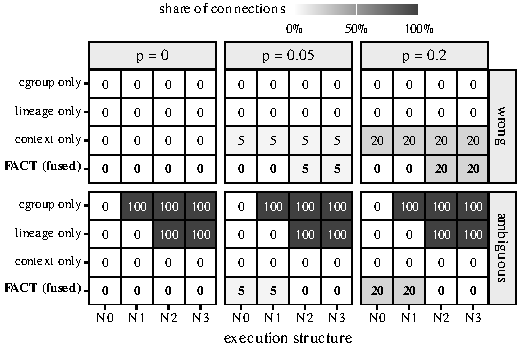
\includegraphics[width=\columnwidth]{generated/fig_e1.pdf}
\caption{E1: percentage of connections credited to the wrong execution (top) or reported as ambiguous (bottom), per resolver, execution structure, and fault fraction $p$ (\EOneRuns\ runs; label: \EOneLabel). Operation modes are pooled; they produced identical counts in every cell.}
\label{fig:e1}
\end{figure}

With correct markers, context-only and fused attribution are correct everywhere, so threads and forked subprocesses inherit the context; mislabeled markers separate them. In N0 and N1, lineage contradicts the label, so the fused resolver flags each mislabeled connection as ambiguous (I/N = 0), whereas context-only credits all of them to the wrong execution. In N2 and N3, both resolvers follow the label, because inside a shared worker no kernel signal can contradict it. The outcome was identical in all \EOneRuns\ confirmatory runs over two boots.

\subsection{Accounting}
The net accounting error hides misattributions, and the decomposition exposes them (Fig.~\ref{fig:acct}). With symmetric mislabels, context-only accounting reports a net error of zero even when a fifth of its connections go to the wrong execution. In N0 and N1, fused accounting moves the mislabeled connections from \emph{wrong} to \emph{uncredited}. Its net error is larger, but it is conservative: across \EOneRuns\ runs, none of the \EOneMislabeled\ mislabeled connections was credited to the wrong execution.

\begin{figure}[!ht]
\centering
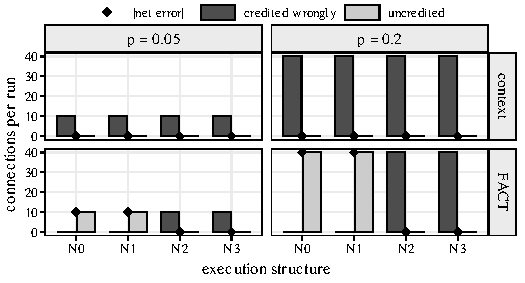
\includegraphics[width=\columnwidth]{generated/fig_acct.pdf}
\caption{E1 accounting with mislabeled markers: connections per run (of 200) credited to the wrong execution or left uncredited, and the absolute net error summed over executions; the remaining connections are credited correctly.}
\label{fig:acct}
\end{figure}

\subsection{Scale and Overhead}

Attribution stays correct and complete up to 64 concurrent executions (E2), and the collector adds microseconds per connection. With $P$ concurrent instances of the closed-loop \texttt{connect} microbenchmark (E2b), capture is complete up to $P{=}4$ (over $10^5$ connections per second); from $P{=}6$ on, with the vCPUs saturated, bpftrace reports lost events, so loss is never silent.

E3 isolates the cost on a closed loop of loopback connections, the worst case for per-connection instrumentation: the collector adds about 8\,$\mu$s to the median \texttt{connect}, and the markers add two failed system calls per operation, costlier when the collector also traces \texttt{openat}. Over the virtual network interface (E3net, \EThreeNetRuns\ runs), the median \texttt{connect} takes \EThreeNetBase\,$\mu$s and the collector adds \EThreeNetAdd\,$\mu$s (\EThreeNetRel\%).

E3b separates the components: attaching the probes while only counting events adds 1.5\,$\mu$s, and exporting one record per connection accounts for most of the remaining 6.7\,$\mu$s, in both the full and the optimized collector. With markers, the optimized variant lowers the added median latency from 19.1 to 14.3\,$\mu$s and the eBPF time per program run from 1304 to 854\,ns. It is a drop-in replacement: rerunning E1 with it (\EOneFastRuns\ runs) reproduced the outcome fractions of the full collector in \EOneFastEqual\ of \EOneFastCells\ cell--resolver combinations.

\subsection{Shared MCP Server}
Thread-keyed context breaks for asynchronous tools; binding the identity to the task fixes it without changing tool code. E4 runs a real MCP server, one process in one cgroup serving $K$ concurrent sessions, so lineage and cgroup are ambiguous for every connection. Synchronous, threaded, and subprocess tools inherit the marker and are attributed correctly; asynchronous tools are not: coroutines of different sessions interleave on the event-loop thread and overwrite its context, so 42\% ($K$=2) and 39\% ($K$=4) of the connections are credited to the wrong session, and connections opened after another coroutine's end marker are ambiguous.

\begin{figure}[t]
\centering
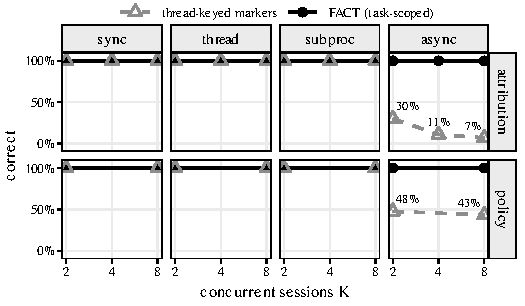
\includegraphics[width=\columnwidth]{generated/fig_e5e6.pdf}
\caption{E5 and E6: correct attribution (top) and correct egress-policy decisions (bottom) in a shared MCP server, per tool type and number of concurrent sessions $K$, with thread-keyed markers (manual) and with the task-scoped binding of \solution{} (fused resolver; \EFiveRuns\ E5 and \ESixRuns\ E6 runs).}
\label{fig:e5e6}
\end{figure}

Figure~\ref{fig:e5e6} (top) compares the two bindings on the same server, tools, and seeds. With manual markers, correct attribution of asynchronous tools falls from 30\% to 7\% as sessions grow, and about 40\% of the connections go to the wrong session at every $K$. With the task-scoped binding, the same tools, without markers, had \EFiveWrongAuto\ errors in \EFiveConnAuto\ connections (a one-sided 95\% Clopper--Pearson bound of 0.2\% at $K{=}8$). Both bindings are correct for the other tools, with median tool-call latencies within 0.2\,ms. Across a real network interface the outcome is the same (E5net and E6net, \EFiveNetRuns\ and \ESixNetRuns\ runs): manual markers fall from \EFiveNetAsyncManMax\% to \EFiveNetAsyncManMin\% correct for asynchronous tools, and the task-scoped binding made \EFiveNetWrongAuto\ errors in \EFiveNetConnAuto\ connections (144 of them identity-less reachability probes, reported as unattributed) and \ESixNetErrAuto\ policy errors in \ESixNetDecAuto\ decisions.

\begin{figure}[t]
\centering
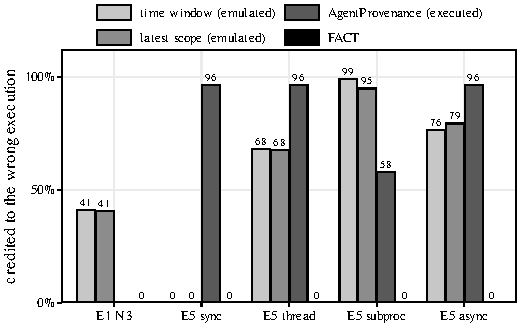
\includegraphics[width=\columnwidth]{generated/fig_baselines.pdf}
\caption{Related systems vs.\ \solution{} in shared workers (E1 N3, $p=0$; E5, $K=8$): percentage of connections credited to the wrong execution. Emulations (\BaseRuns\ runs) use the manual-mode call boundaries; AgentProvenance was executed in the E5 rounds (E5ap).}
\label{fig:base}
\end{figure}

\subsection{Comparison with Related Mechanisms}
Time-based and latest-binding correlation cannot separate concurrent tool calls inside one process; \solution{} can. We emulate the documented mechanisms of related systems as offline resolvers over the same logs, with process lineage first and the tool-call boundaries of the manual mode (Fig.~\ref{fig:base}): the \emph{time-window} resolver picks the latest tool-call start within 500\,ms, as in AgentSight, and the \emph{latest-scope} resolver picks the open binding that started last, as in AgentProvenance. With distinct process trees (N0, N1), lineage alone suffices. Inside a shared worker, time separates only blocking calls: both misattribute 41\% of the connections in N3 and 68--99\% for threaded, subprocess, and asynchronous tools with eight sessions.

Running AgentProvenance itself confirms the mechanism and shows the emulation was optimistic (E5ap, \APRuns\ runs). With four and eight sessions it credited \APWrongMin--\APWrongMax\% of the connections of synchronous, threaded, and asynchronous tools to the wrong session (\APWrongTwoMin--\APWrongTwoMax\% with two), and \APSubMin--\APSubMax\% for subprocess tools, whose child processes it can sometimes match; \solution{} misattributed \APAgentnetWrong\ of \APAgentnetConn\ connections in the same rounds. Its harness sees each call's window from the client, so when a tool connects all $K$ windows are open and it picks the latest. AgentSight attributes per process, so in a shared server it cannot name a session; we keep it emulated.

\subsection{Egress Policy and LLM Agents}
Binding errors turn into policy errors in both directions, and the task-scoped binding removes them. With manual markers and asynchronous tools, only 48\% ($K$=2) and 43\% ($K$=8) of the decisions are correct (Fig.~\ref{fig:e5e6}, bottom): mislabeled restricted executions pass (9--11\% false allows, \ie bypasses) and others are blocked (42--48\% false denies). With the task-scoped binding, all \ESixDecAuto\ decisions match the reference. Connections without identity are denied by default, so a missing binding fails closed instead of inheriting a guess.

In E7 the tool calls are chosen by a language model. Four agents share one MCP server process in one cgroup; the fused resolver attributed \ESevenWrong\ of \ESevenConn\ connections incorrectly, and the policy made \ESevenDecOK\ correct decisions out of \ESevenDec. The median tool call took \ESevenToolMs\,ms, against several seconds per model step. With larger models on a GPU and up to eight agents (E7m, \ESevenMRuns\ runs), the result is the same: \ESevenMWrong\ of \ESevenMConn\ connections were misattributed, and \ESevenMDecOK\ of \ESevenMDec\ policy decisions were correct. Commercial models from Anthropic and OpenAI agree (\ESevenCRuns\ runs each): with Claude (E7c), \ESevenCWrong\ of \ESevenCConn\ connections misattributed and \ESevenCDecOK\ of \ESevenCDec\ decisions correct; with GPT (E7o), \ESevenOWrong\ of \ESevenOConn\ and \ESevenODecOK\ of \ESevenODec, for US\$\,\ESevenCUSD\ and US\$\,\ESevenOUSD\ in API tokens. Replayed without the models (E7r), \ESevenRSame\ of \ESevenRRuns\ runs reproduced the same calls and outcomes, so the results do not depend on the models staying available.

\begin{table}[t]
\centering
\caption{Binding faults injected into the framework: a fraction $p$ of each execution's tool calls carries another execution's identity (task-scoped binding; tools pooled; \FaultEfiveRuns\ E5f, \FaultEsixRuns\ E6f, and \FaultEsevenRuns\ E7f runs). Wrong: mislabeled connections credited to the wrong execution; other err.: errors on correctly labeled calls.}
\label{tab:fault}
\footnotesize
\setlength{\tabcolsep}{2.2pt}
\IfFileExists{generated/tab_fault.tex}{% gerado por analysis/fault_tables.py — não editar à mão
\begin{tabular}{@{}lrrrrrrr@{}}
\toprule
 & & \multicolumn{3}{c}{attribution (E5f)} & \multicolumn{3}{c}{policy (E6f, E7f)} \\
\cmidrule(lr){3-5}\cmidrule(l){6-8}
$K$ & $p$ & mislab. & wrong & other err. & FA & FD & other err. \\
\midrule
2 & 0.04 & 64 & 64 & 0 & 16 & 32 & 0 \\
2 & 0.20 & 320 & 320 & 0 & 80 & 160 & 0 \\
8 & 0.04 & 256 & 256 & 0 & 72 & 64 & 0 \\
8 & 0.20 & 1280 & 1280 & 0 & 208 & 480 & 0 \\
\midrule
\multicolumn{2}{l}{E7f (LLM)} & 104 & 0 & 0 & 0 & 86 & 0 \\
\bottomrule
\end{tabular}
}{\TBD}
\end{table}

\begin{table}[t]
\centering
\caption{E6L: policy decisions with mislabeled calls when executions have their own process trees (N0 and N1, both operation modes pooled; \LinRuns\ confirmatory runs over two boots). Conflicts: contradictions between label and process tree flagged in the kernel.}
\label{tab:lineage}
\footnotesize
\setlength{\tabcolsep}{2.4pt}
\IfFileExists{generated/tab_lineage.tex}{% generated by analysis/fault_tables.py; do not edit by hand
\begin{tabular*}{\columnwidth}{@{\extracolsep{\fill}}lrrrrrr@{}}
\toprule
Lineage check & $p$ & decisions & mislab. & conflicts & FA & FD \\
\midrule
label only & 0.05 & 3200 & 160 & -- & 48 & 80 \\
label only & 0.20 & 3200 & 640 & -- & 144 & 320 \\
deny on conflict & 0.05 & 3200 & 160 & 160 & 0 & 112 \\
deny on conflict & 0.20 & 3200 & 640 & 640 & 0 & 496 \\
tree owner & 0.05 & 3200 & 160 & 160 & 0 & 0 \\
tree owner & 0.20 & 3200 & 640 & 640 & 0 & 0 \\
\bottomrule
\end{tabular*}
}{\TBD}
\end{table}

\subsection{Faulty Bindings}

A faulty label affects only its own call, and wherever executions have their own process trees, the in-kernel lineage check stops the bypasses it would cause. In the shared MCP server (Table~\ref{tab:fault}), every mislabeled connection is credited to the execution named by the label (\FaultMisWrong\ of \FaultMis), and no other connection or decision is affected (\FaultSpill\ errors elsewhere): because the identity is bound to the task, a faulty call does not contaminate later calls. No kernel signal contradicts a label inside one process, so \FaultPolErrPct\% of the mislabeled calls also became policy errors, in both directions. The LLM agents have disjoint allow-lists, so \FaultEsevenAllowed\ of their \FaultEsevenMis\ mislabeled calls were allowed: the fault failed closed. Where executions have their own process trees, the lineage check moves the offline detection of contradicted labels (E1) into the kernel (Table~\ref{tab:lineage}). With the label alone, the policy decided \LinModeZeroPct\% of the mislabeled connections wrongly. Denying on conflict removed every false allow, and deciding by the tree owner removed every decision error (\LinModeTwoErr\ in \LinModeTwoDec\ decisions); in both modes, the conflicts flagged in the kernel were exactly the mislabeled connections. In the shared server, where the tree is shared and therefore not registered, the check vetoed none of \LsDecisions\ correct decisions (E6Ls).

Finally, \texttt{factd}, fed the recorded collector streams in arrival order with a 100\,ms reordering window, reproduced the per-execution credited, ambiguous, and unattributed counts of the offline evaluation in \AgentnetdEqual\ of \AgentnetdRuns\ runs.

% ===== 07-discussion.tex =====
\section{Discussion and Limitations}
\label{sec:discussion}
\textbf{Asynchronous tools.} Thread-keyed context fails silently for coroutines that yield between markers (E4), and no kernel signal can detect it inside one thread. Binding the identity to the task and handing it to the kernel at the system call that creates the connection or process removes the failure (E5) without changing tool code. The approach relies on the runtime propagating task context, which Python's \texttt{asyncio} and \texttt{anyio} provide through context variables (\texttt{contextvars}); equivalent mechanisms exist in other runtimes (e.g., asynchronous local storage in Node.js), but we implemented and evaluated only Python.

\textbf{Threat model and trust.} The identity is asserted by the agent runtime, which we trust as the operator's component; tools and MCP clients are not trusted. In the prototype, this trust is not enforced: any process can emit a marker, and the \texttt{\_meta} identity is chosen by the client, so a malicious tool or client could claim another execution's identity. The policy is therefore a containment control for correct or buggy runtimes, not a security boundary against adversarial tools. Hardening is straightforward to specify but not evaluated here: accept markers only from registered runtime threads, freeze a process's identity at \texttt{exec}, and derive the identity from an authenticated MCP session instead of \texttt{\_meta}. The fused resolver bounds a faulty label only where the process structure is informative, and the policy's lineage check enforces the same bound in the kernel; in shared workers the remaining defenses are outside the kernel, e.g., auditing the runtime or isolating executions in separate processes. Deciding by the tree owner assumes that a registered tree is never handed over to another execution; denying on conflict makes no such assumption, which is why it is the default. A related limitation is that the per-thread entry is not cleared after a call, so a connection opened by native code that bypasses the wrappers inherits the last identity set on that thread.

\textbf{Threats to validity.} We follow the categories of Wohlin et al.~\cite{wohlin2012experimentation}. \emph{Internal:} capture loss, socket-pointer reuse in the connect/state join, and PID reuse (not exercised). \emph{Construct:} synthetic executions approximate, but are not, tasks or tool calls; attribution is evaluated for TCP connection attempts, not bytes, and pooled or reused connections (e.g., HTTP keep-alive shared across sessions) are not exercised; such reuse would credit later requests to the session that opened the connection. \emph{External:} a single kernel and host, a VMware virtual machine without CPU frequency control; loopback traffic; IPv4 only; one MCP SDK version; a single small local model in E7, whose tool-call behavior is part of the workload rather than a controlled factor. \emph{Conclusion:} events within a run are dependent, so statistics are computed over runs.

\textbf{Scope.} We attribute and police TCP connection attempts; byte-level accounting per execution and policies over destinations other than ports are natural extensions of the same identity. Like the accounting, the policy relies on the runtime-provided identity only where lineage cannot contradict it, i.e., inside a shared worker; there, attribution is runtime-asserted rather than kernel-verified and should be reported as such.

\section{Conclusion and Future Work}
\label{sec:conclusion}

Inside a shared worker, attribution and policy fail silently unless the identity of the execution reaches the kernel. \solution{} hands it to the kernel when a connection or process is created and fuses it with lineage and cgroups. With correct labels it made no attribution or policy error in any confirmatory run, with asynchronous tools, a real network interface, and LLM agents driven by open and commercial models, where an executed related system misattributed most connections; faulty labels become reported ambiguity where the process structure is informative. The cost is microseconds per connection.

Future work includes deriving the identity from authenticated MCP sessions; extending attribution to bytes, reused connections, IPv6, User Datagram Protocol (UDP) traffic, and other runtimes; aggregating counters in the kernel; extending the same identity to the LLM tokens each execution consumes, enabling per-execution budgets; exporting records through IPFIX and OpenTelemetry; and evaluating \solution{} across physical hosts and with network management agents for beyond-5G and 6G operation~\cite{corici2025agents,xiao2025agentic}.


\bibliographystyle{IEEEtran}
\bibliography{references}
\end{document}
